%%%%%%%%%%%%%%%%%%%%%%%%%%%%%%%%%%%%%%%%%
% University Assignment Title Page 
% LaTeX Template
% Version 1.0 (27/12/12)
%
% This template has been downloaded from:
% http://www.LaTeXTemplates.com
%
% Original author:
% WikiBooks (http://en.wikibooks.org/wiki/LaTeX/Title_Creation)
%
% License:
% CC BY-NC-SA 3.0 (http://creativecommons.org/licenses/by-nc-sa/3.0/)
% 
% Instructions for using this template:
% This title page is capable of being compiled as is. This is not useful for 
% including it in another document. To do this, you have two options: 
%
% 1) Copy/paste everything between \begin{document} and \end{document} 
% starting at \begin{titlepage} and paste this into another LaTeX file where you 
% want your title page.
% OR
% 2) Remove everything outside the \begin{titlepage} and \end{titlepage} and 
% move this file to the same directory as the LaTeX file you wish to add it to. 
% Then add \input{./title_page_1.tex} to your LaTeX file where you want your
% title page.
%
%%%%%%%%%%%%%%%%%%%%%%%%%%%%%%%%%%%%%%%%%
%\title{Title page with logo}
%----------------------------------------------------------------------------------------
%	PACKAGES AND OTHER DOCUMENT CONFIGURATIONS
%----------------------------------------------------------------------------------------

\documentclass[12pt]{article}
\usepackage[english]{babel}
\usepackage[utf8x]{inputenc}
\usepackage{amsmath}
\usepackage{graphicx}
\usepackage[colorinlistoftodos]{todonotes}
\usepackage{amsfonts}
\usepackage{algorithm}
\usepackage{algpseudocode}
\usepackage{listings}
\usepackage{float}

\newcommand{\vect}{\mathbf}
\newcommand{\nul}{\operatorname{Nul}}
\newcommand{\col}{\operatorname{Col}}
\newcommand{\row}{\operatorname{Row}}


\textheight=240truemm \textwidth=160truemm 
\hoffset=-10truemm \voffset=-30truemm

\begin{document}

\begin{titlepage}

\newcommand{\HRule}{\rule{\linewidth}{0.5mm}} % Defines a new command for the horizontal lines, change thickness here

\center % Center everything on the page
 
%----------------------------------------------------------------------------------------
%	HEADING SECTIONS
%----------------------------------------------------------------------------------------

\textsc{\LARGE Ukrainian Catholic University}\\[1cm] % Name of your university/college
\textsc{\Large  Faculty of Applied Sciences}\\[0.5cm] % Major heading such as course name
\textsc{\large Data Science Master Programme}\\[0.5cm] % Minor heading such as course title
%----------------------------------------------------------------------------------------
%	TITLE SECTION
%----------------------------------------------------------------------------------------
\vspace*{1cm}

\HRule \\[0.4cm]
{ \huge \bfseries Image compression using Linear Algebra: SVD and DCT}\\[10pt]
{\Large \bfseries Linear Algebra final project report}\\[0.4cm] % Title of your document
\HRule \\[1cm]
 
%----------------------------------------------------------------------------------------
%	AUTHOR SECTION
%----------------------------------------------------------------------------------------
\vspace*{1cm}

% If you don't want a supervisor, uncomment the two lines below and remove the section above
\Large \emph{Authors:}\\
Dmytro \textsc{Nadobko}\\ Yevhen \textsc{Stepanov}\\ Dmytro \textsc{Rudenko}\\ [1cm] % Your name

%----------------------------------------------------------------------------------------
%	DATE SECTION
%----------------------------------------------------------------------------------------
\vspace*{1cm}
{\large 31 January 2022}\\[2cm] % Date, change the \today to a set date if you want to be precise

%----------------------------------------------------------------------------------------
%	LOGO SECTION
%----------------------------------------------------------------------------------------


\includegraphics[height=5cm]{UCU-Apps.png}\\[1cm] % Include a department/university logo - this will require the graphicx package
 
%----------------------------------------------------------------------------------------

\vfill % Fill the rest of the page with whitespace

\end{titlepage}

\begin{abstract}
The aim of research is to investigate two different approaches for image compression based on Singular Value Decomposition (SVD) and Discrete Cosine Transform (DCT), compare complexity and quality of each approach, provide cases where each approach show its best results.
\end{abstract}

\section{Introduction}

Image compression is minimizing the size in bytes of a graphics file without degrading the quality of the image to an unacceptable level. The reduction in file size allows more images to be stored in a given amount of disk or memory space. It also reduces the time required for images to be sent over the Internet or downloaded from Web pages. 

Its first major use case in during the 1960s when satellites used it to transfer images from space to Earth.  It has become even more useful since the implementation of the internet, as smaller sizes
became much more important to a media that demanded instant access. The most common use
today is in streaming websites like Youtube, Netflix, and Hulu, where 60 images or more are
sent in a single second over the internet. Without image compression, ridiculous internet speeds
would be needed to do this, but compression allows for up to 10 times less data to be sent in
order to get the same picture.

One of the simplest ways to store an image is in the Raster format, which is essentially an
$M \times N$ matrix storing the values of each pixel, where m and n are the length and width of the
image. For a colored image, the same is done but with three matrices, each one holding the red,
green, or blue pixel values for the RGB format. The main linear algebra compression algorithms
use this common method of storing images, as it is quite nice to have a matrix when dealing in
linear algebra.

One important aspect of image compression is whether it is lossy or lossless. A lossy
compression results in some information being lost in the compression, but allows for a more
effective compression. A lossless compression stores all of the same information, but just in a
compressed state. Usually, the lossless compressions mostly rely on storing bytes differently and
don’t really apply linear algebra. However, lossy compressions apply multiple linear algebra
techniques, including the entire process of SVD and various matrix transformations in the DCT.

\section{Problem Setting}

\subsection{Image Compression Problem}

In the field of Image processing, the compression of images is an important step before we start the processing of larger images or videos. The compression of images is carried out by an encoder and output a compressed form of an image. In the processes of compression, the mathematical transforms play a vital role. 

The general representation of the image in a computer is like a vector of pixels. Each pixel is represented by a fixed number of bits. These bits determine the intensity of the color - on gray-scale if a black and white image and has three channels of RGB (red, green, blue) if colored images.

Consider a color image that has a 4K resolution of $3840 * 2160$ pixels and each pixel uses $8 * 3 = 24$ bits (as color images has 3 channels) to represent the intensity. So the total number of required bits  is equal to $3840 * 2160 * 24 = 199,065,600$ bits per image. And consider if it is a video with 60 FPS (frames per second) of the above-mentioned type images then the total bits for a video of 3 secs is: $3 * 60 * 199,065,600 = 35,831,808,000$ bits, that is actually $4.17137146$ gigabytes. 

As we see just to store a 3-sec video we need so many bits which is very huge. If there isn't image compression, Netflix 4K movie with average duration in 97 minutes would require $\sim 23.7$ terabytes, so it will take $23$ days $26$ minutes and $12$ seconds for downloading with $100$ MB/sec speed.
So, we need a way to have proper representation as well to store the information about the image in a minimum no of bits without losing the character of the image. Thus, image compression plays an important role. 

\subsection{Hypothesis}

We are proposing a scheme for the image compression using discrete cosine transform and singular value decomposition.
The effort is made to compare the metrics for SVD and DCT in terms of compression ratio, SSIM, PSNR and time complexity.
The experiment is done for different set of pictures. 
Visually we can compare the results of two approaches and approve the hypothesis that the results after compression of DCT has less noise than the ones of SVD.
Today JPEG is very popular as a data format. But it is not really a data format. It is an compression method. There are many compression method and JPEG is one of them. 

The way that the discrete cosine transform works, is we take some data, in this case, our image data, and we try to represent it as the sum of lots of cosine waves. It transfers an image from the spatial domain to a frequency domain.
The DCT can be used to convert the signal (spatial information) into numeric data ("frequency" or "spectral" information) so that the image's information exists in a quantitative form that can be manipulated for compression.    
The signal for a graphical image can be thought of as a three-dimensional signal.

It became popular thanks to the algorithm DCT. All these steps written above show the reason why JPEG algorithm is so popular nowadays.

\subsection{Quality Evaluation}

Once we have developed a compression algorithm, we need to be able to measure its performance. Because of the number of different areas of application, different terms have been developed to describe and measure the performance. 

The basic metric to measure the difference between the decompressed and the original image is the Frobenius norm, but since it directly depends on the size of the image matrix, we must look at the difference per pixel, which turns the Frobenius norm into the mean squared error. But despite this, such a metric can only serve for a theoretical evaluation of our algorithm, since we want to compress images as efficiently as possible and so that a person does not see significant differences between the pictures, it makes sense to introduce a method that will provide such a measurement.

The Structural Similarity Index (SSIM) is a perceptual metric that quantifies image quality degradation caused by processing such as data compression or by losses in data transmission. It is a full reference metric that requires two images from the same image capture — a reference image and a processed image. Structural information is the idea that the pixels have strong inter-dependencies especially when they are spatially close. These dependencies carry important information about the structure of the objects in the visual scene. Luminance masking is a phenomenon whereby image distortions (in this context) tend to be less visible in bright regions, while contrast masking is a phenomenon whereby distortions become less visible where there is significant activity or "texture" in the image.

The SSIM index is calculated on various windows of an image. The measure between two windows $x$ and $y$ of common size $N \times N$ is: $$ SSIM(x, y)=\frac{(2\mu_x\mu_y + c_1)(2 \sigma_{xy} + c_2)}{({\mu_x}^2 + {\mu_y}^2 + c_1)({\sigma_x}^2 + {\sigma_y}^2 + c_2)} $$ with:

\begin{itemize}
  \item $\mu_x$ the average of $x$
  \item $\mu_y$ the average of $y$
  \item ${\mu_x}^2$ the variance of $x$
  \item ${\mu_y}^2$ the variance of $y$
  \item $\mu_{x y}$ the co-variance of $x$ and $y$
  \item $c1 = {(K_1 L)}^2 , c2 = {(K_2 L)}^2$ two variables to stabilize the division with weak denominator
  \item $L$ the dynamic range of pixel-values (typically this is $2^{bps} - 1, bps = $ bits per pixel)
  \item $k_1 = 0.01$ and $k_2 = 0.03$ by default
\end{itemize}

The SSIM formula is based on three comparison measurements between the samples of $x$ and $y$: luminance ($l$), contrast ($c$) and structure ($s$). The individual comparison functions are:

$$ l(x, y) = \frac{2\mu_x\mu_y + c_1}{{\mu_x}^2 + {\mu_y}^2 + c_1} $$
$$c(x, y) = \frac{2\sigma_x\sigma_y + c_2}{{\sigma_x}^2 + {\sigma_y}^2 + c_2}$$
$$ s(x, y)=\frac{\sigma_{x y} + c_3}{\sigma_x\sigma_y + c_3}, c_3 = c_2 / 2 $$

SSIM is a weighted combination of those comparative measures:

$$SSIM(x,y)=[l(x,y)^\alpha \cdot c(x,y)^\beta \cdot s(x,y)^\gamma]$$

Setting the wights $\alpha, \beta, \gamma$ to $1$ and the formula can be reduced to the form shown above.

\subsection*{Data set description}

After measurement approach is chosen, data with images is needed for testing. Since needed images should be raw (without compressing), PPM image format was chosen. PPM stands for Portable Pixel Map. This format is a convenient and simple way to save image data. It is true that GIF, PNG and JPG are more commonly found. However, there are many good image manipulation programs to convert between the various formats. The more common formats noticed before use data compression to reduce file sizes, so they are not suitable for our problem. PPM is a very simple format that allows very easy reading and writing of image files.

\begin{figure}[H]
  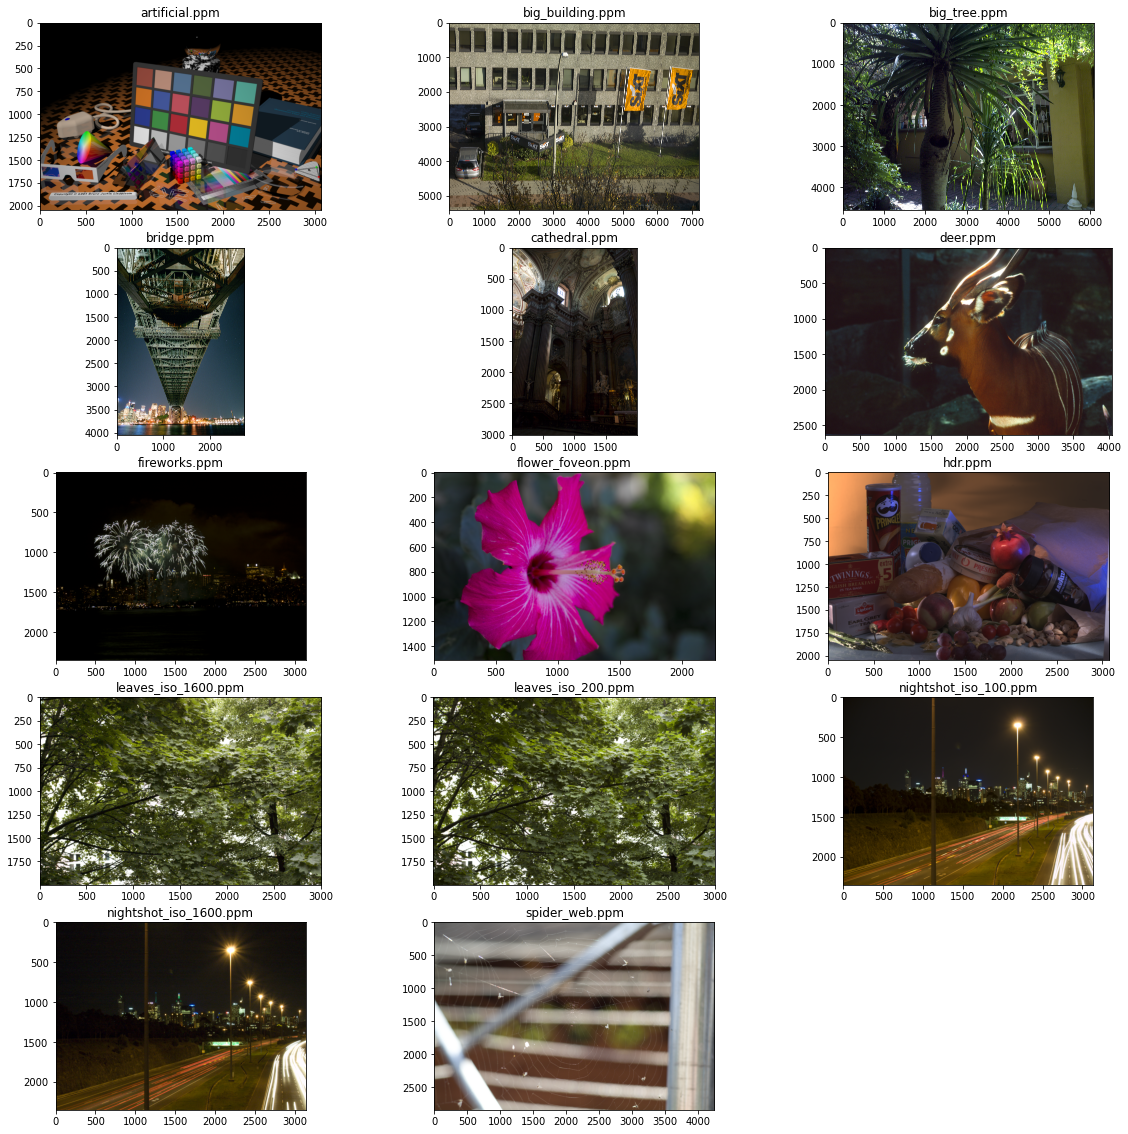
\includegraphics[width=\linewidth]{data_set.png}
  \caption{Test data set}
  
  \label{fig:data_set}
\end{figure}

The data set shown at Figure \ref{fig:data_set} and consists of 14 different pictures, most of them are camera shots, but there is also a picture generated by a computer using ray tracing technology (artificial.ppm). The data set contains both images taken during the daytime and at night. Image resolution varies from $2000 \times 3008$ pixels to $5412 \times 7216$ pixels.

There are also pictures taken at night and during the day, but at the same time made with low and high ISO settings. In very basic terms, ISO is simply a camera setting that will brighten or darken a photo. As ISO number is increased, photos will grow progressively brighter (illustrated at Figure \ref{fig:iso_example}). For that reason, ISO can help to capture images in darker environments.

\begin{figure}[H]
  \centering
  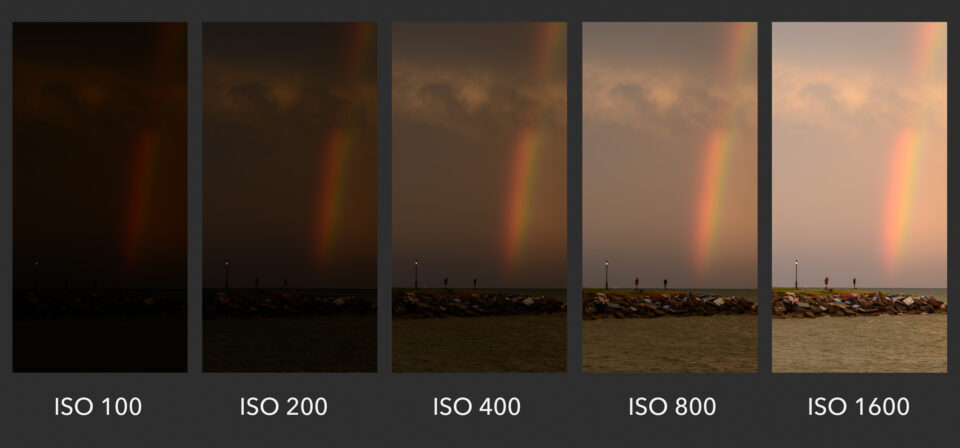
\includegraphics[width=.8\linewidth]{ISO-brightness-chart-960x448.jpeg}
  \caption{ISO change example}
  \label{fig:iso_example}
\end{figure}

However, raising your ISO has consequences showed at Figure \ref{fig:iso_noise}. A photo taken at too high of an ISO will show a lot of grain, also known as noise, and might not be usable. So, brightening a photo via ISO is always a trade-off.

\begin{figure}[H]
  \centering
  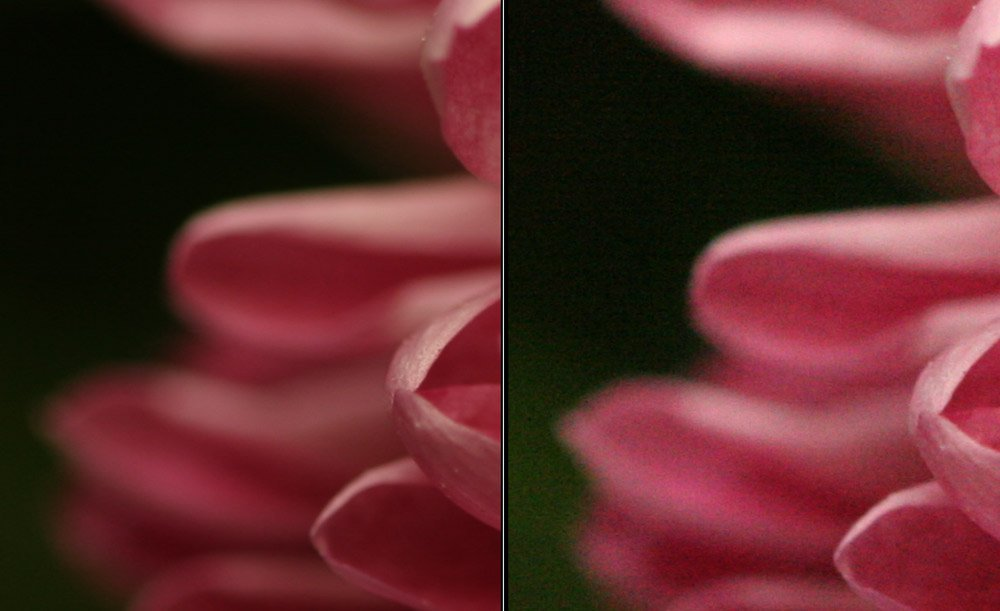
\includegraphics[width=.8\linewidth]{iso-1.jpeg}
  \caption{ISO 100 and ISO 3200 noise}
  \label{fig:iso_noise}
\end{figure}

\section{Solution Description}

\subsection{Singular Value Decomposition}

The Singular Value Decomposition (SVD) is used in linear regression and least square methods, and can be a useful technical tool for solving linear systems without unique solution (Moore-Penrose pseudoinverse), calculating low-rank approximations, performing principal component analysis (PCA). There is also a lot of real world applications of SVD such as image compression, recommendations systems, numerical weather forecast or natural language processing.

Let $A \in \mathbb{R}^{n \times m}$ be an arbitrary (not necessarily a square) matrix. It can be complex valued as well, but in the examples we are going to deal with real matrices only. Then there exist matrices $U \in \mathbb{R}^{n \times n}$, $D \in \mathbb{R}^{n \times m}$ and $V \in \mathbb{R}^{m \times m}$, such that $$ A = U D V^*, $$ where $U$ and $V$ are unitary matrices, that is $U^*U = U U^* = I_n$ and $V^*V=V V^*=I_m$ and $D$ is a diagonal matrix, that is $d_{i j}=0$ if $i \ne j$. The star operation means conjugate transpose, that is $(V^*)_{i j} = \overline V_{j i}$, but since we are dealing with real matrices now, this is the same as the transpose of the matrix. The diagonal elements in $D$ are non-negative numbers, in decreasing order: $d_{ii} = \sigma_i$, $\sigma_1 \geq \sigma_2 \geq \ldots \geq \sigma_r > \sigma_{r+1} = \ldots = \sigma_{\min(n,m)} = 0$, where $r$ is the rank of the matrix $A$. These $\sigma$ values in the diagonal of $D$ are called the singular values of $A$.

\subsection*{Low-rank approximation}

Let $k \in \mathbb{N}$ a given natural number, where $k \leq \text{rank}(A) \leq \min \{n, m\}$. What we look for is a matrix $A_k$ having $ \text{rank}(A_k) = k$ which is the best approximation of $A$ among the matrices that have rank equals to $k$. To formulate the low-rank approximation problem, we would like to solve the following minimization problem: $$ \| A - B \|_F \to \min !\qquad \mbox{ subject to } \quad B \in \mathbb{R}^{n \times m},  \text{rank}(B) = k. $$ Here $\| X \|_F$ denotes the Frobenius norm of a matrix $X$ which is the square root of the sum of squares of the elements of $X$.
    
The solution of this problem can be obtained from the SVD-decomposition of $A$. If $A = U D V^*$, then we keep the first $k$ values in $D$ as is and set the subsequent singular values to zero. Let us denote the resulting diagonal matrix by $D_k$. It is easy to see that we only have to keep the first $k$ columns of $U$ and the first $k$ rows of $V$, since their other columns would be multiplied by zeros anyway. To sum up, the matrix $A_k := U_k D_k V_k^*$ is the closest matrix to $A$ (in Frobenius norm) having rank $k$, where $U_k$ and $V_k$ consist of the first $k$ columns and rows of $U$ and $V$, respectively.

Actually, in our problem image is represented as a large matrix $A$, that has large dimensions $n,m$  and $k$ is relatively small, then the information we need to store to approximate the information content stored in $A$ is much smaller. That is, we can reduce the storage space significantly and we are still able to store almost the same information that the original matrix has.

\subsection{Discrete Cosine Transform}
A discrete cosine transform (DCT) expresses a finite sequence of data points in terms of a sum of cosine functions oscillating at different frequencies.

DCT is a transformation that uses matrix multiplications to compress matrix data. First, the image is split into many $N \times N$ matrices, with the ideal number for $N$ usually being $8$. Then, an $N \times N$ transformation matrix is created using a cosine formula based on the $i, j$ positions in the matrix. Each $N \times N$ square of the image is then left multiplied by this matrix, and right multiplied by the transpose of the matrix. 

$$D = TMT^T$$

After this process, there are different $N \times N$ quantization matrices ranging from compression percentages $0-100\%$ that can be used to compress each transformed matrix.

The use of cosine rather than sine functions is critical for compression, since it turns out (as described below) that fewer cosine functions are needed to approximate a typical signal, whereas for differential equations the cosines express a particular choice of boundary conditions. In particular, a DCT is a Fourier-related transform similar to the discrete Fourier transform (DFT), but using only real numbers.

The DCT-II, also known as simply the DCT, is the most important image compression technique. It is used in image compression standards such as JPEG, and video compression standards such as H.26x, MJPEG, MPEG, DV, Theora and Daala. There, the two-dimensional DCT-II of $N \times N$ blocks are computed and the results are quantized and entropy coded. In this case, $N$ is typically $8$ and the DCT-II formula is applied to each row and column of the block. The result is an $8 \times 8$ transform coefficient array in which the $(0,0)$ element (top-left) is the DC (zero-frequency) component and entries with increasing vertical and horizontal index values represent higher vertical and horizontal spatial frequencies.

\section{Implementation}

\subsection{SVD}

Since Singular Value Decomposition mostly works with 2D matrices, the first thing is needed to do is divide our image into 3 matrices, each corresponding to one of the RGB (red, green, blue) channels and normalize the pixel space (using 8-bit format is $[0, 256)$) to $[0, 1]$ float space. The result of dividing presented at Figure \ref{fig:rgb}

\begin{figure}[H]
  \centering
  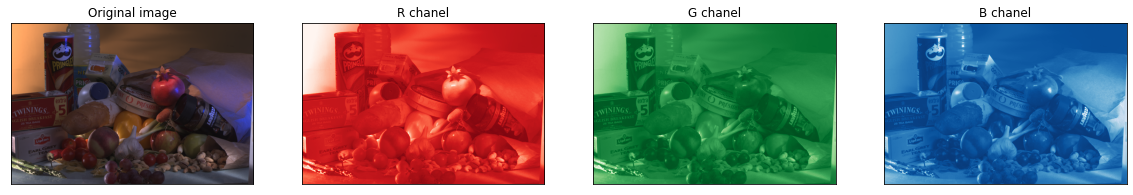
\includegraphics[width=\linewidth]{rgb_chanels.png}
  \caption{RGB channels}
  \label{fig:rgb}
\end{figure}

After this pre-processing is done, performing SVD algorithm to each of three images is the next step. SVD algorithm in a nutshell is a problem of finding eigenvalues and eigenvectors, because SVD decompose matrix $A_{n \times m}$ into three matrix: $U_{n \times n}$, $d_{n \times m}$, ${V^T}_{m \times m}$, where:

\begin{itemize}
  \item $U_{n \times n}$ is matrix of the orthogonal eigenvectors of $AA^T$
  \item $d_{n \times m}$ diagonal matrix of singular values that are square roots of eigenvalues of $A^TA$ 
  \item ${V^T}_{m \times m}$ is transpose of matrix containing orthogonal eigenvectors of $A^TA$
\end{itemize}

Important notice, that now there are 9 matrices (3 per each channel) with total size $3 \times (n \times n + m \times m + min(n, m))$ bytes, as initial image can be stored using $n \times m \times 3$ bytes, there is need for additional space more than image size for processing compression. After it's done there is no needs in any additional space.

Last step in compression pipeline is k-rank approximation, that consists of reducing elements, except the first $k$ rows from top of the matrix $U$, the first $k$ eigenvalues from $d$, and the first $k$ columns from left of the matrix $V$. So, the new matrix $U, d, V$ will have following dimensions: $n \times k, k \times k, k \times m$ respectively. Also, as $d$ is diagonal matrix, there is possibility to store vector of eigenvalues, instead of explicitly store the whole matrix.

Now, image finally compressed and could be store in terms of these 9 reduced matrix. Compressed size can be calculated as $3 \times (n \times k + k + k \times m)$. As $k$ is much smaller than $n$ and $m$, good compression rate without significant loss of quality could be achieved.

When it's time to decompress image, reconstruction process is quite simple, as we made decomposition of matrix $A = U d V^T$, there is need to just multiply reduced matrix in correct order. Result of multiplying will be 3 channels, as compressed image's stored in such format. The final stage is to composite RGB layers back to get reconstructed image. 


\begin{figure}[H]
  \centering
  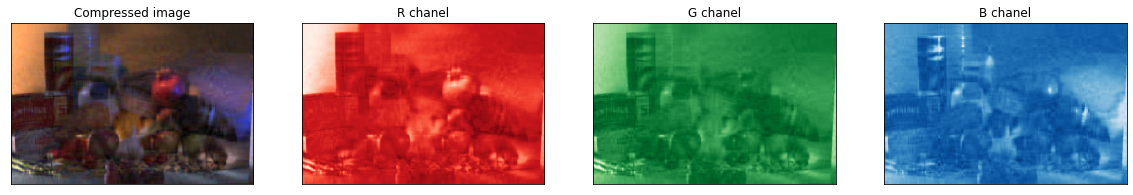
\includegraphics[width=\linewidth]{rgb_compressed.png}
  \caption{Decompressed image and layers}
  \label{fig:rgb_com}
\end{figure}

At Figure \ref{fig:rgb_com} showed reconstructed channels and final image. Parameter $k$ is equal to $20$, initial size of picture is $150,994,944$ bytes, of compressed image is $2,458,080$ bytes, so compression rate is $\sim 1.62\%$, also during compression process it was taken $327,204,864$ bytes of additional space to perform SVD. 

Below there is a complete description of the compression and decompression process, as well as calculating the compression rate using pseudocode.

\begin{algorithm}[H]
\caption{Image compression and decompressing process using SVD}\label{alg:svd}
\begin{algorithmic}
\State originalBytes \gets image.nbytes$
\State image \gets image / 255$
\State image_{red}, image_{green}, image_{blue} \gets divideByChannel(image)$
\State U, d, V \gets constructSvdForRgbChannels(image_{red}, image_{green}, image_{blue})$
\State matrix \gets [U,  d, V]$
\State bytesToBeStored \gets 0$
\For{$i \gets 0$ to $matrix$}             
    \State bytesToBeStored += matrix.nbytes
\EndFor
\State U,  d, V  \gets kRankApproximationForRgb()$
\State matrix \gets [U,  d, V]$
\State compressedBytes \gets 0$
\For{$i \gets 0$ to $matrix$}  
    \State compressedBytes += matrix.nbytes
\EndFor
\State ratio \gets compressedBytes / originalBytes$
\State imageApprox_{RGB} \gets  approximatedMatrixForRgbChannels$
\State reconstructedImage \gets imageReconstruction(
      imageApprox_{RGB}, 
      image.shape)$
\end{algorithmic}
\end{algorithm}

Also, at Figure \ref{fig:com} presented comparing between original and decompressed image:

\begin{figure}[H]
  \centering
  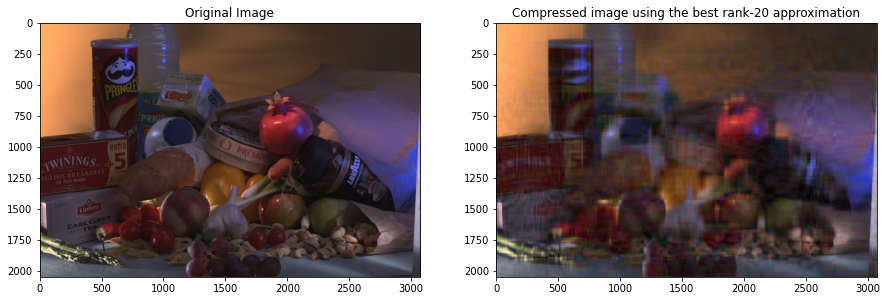
\includegraphics[width=\linewidth]{comparsion.png}
  \caption{Original and compressed images using SVD}
  \label{fig:com}
\end{figure}

\subsection{DCT}

Just like SVD, Discrete Cosine Transform method is applied to 2D matrices, so the first step is the same. The image should be divided into 3 matrices, by each color. The result of dividing can be seen in Figure \ref{fig:rgb}. 

After these steps the direct DCT algorithm is applied to each matrix. The principle behind the DCT algorithm is that any matrix $N \times M$ size can be described as a combination of $N \times M$ cosine functions with different parameters. The DCT algorithm is applied to vectors. So we take each line of image and apply the following formula.

$$ X_{k}=\sum_{n=0}^{N-1} x_{n} \cos \left[\frac{\pi}{N}\left(n+\frac{1}{2}\right) k\right] \quad \text {, for } k=0, \ldots N-1 $$

$$ X_{0}=\sqrt{\frac{1}{2}}X_{0} $$

$$ X_{k}=\sqrt{\frac{2}{N}}X_{k} \text {, for k = 0,...N - 1, where N is the size of a line vector}$$ 

Afterwards, the same formula is applied to each column vector of the image.
Gotten result is the matrix A of size $N \times M$, each element of which is describing the contribution of a specific cosine function with different parameters. Having this matrix also provide information which cosine functions have the most contribution to our image. There are several approaches for it. The one using quantization tables. This approach is used by JPEG compression. The approach in our implementation is more trivial, but also shows good results. We set the compression rate, giving the maximum number of used cosine functions, and select $**z**$ biggest values from matrix $A$. Most parameters from the upper left corner are appearing as they are related to cosine functions with the longest period, which is more common in the image and describe big details.
Now as the image is finally compressed it is stored in $3 \times z \times 3$ ($3$ colors, $z$ parameters, and $3$ parameters of data $x$, $y$, and cosine coefficient). These matrices is named B in the following notations.

When it is time to decompress the decompressed A matrices are formed from our B matrices. And then the next formula is applied for each column:

$$ X_{0}=\sqrt{\frac{1}{2}}X_{0} $$

$$ X_{k}=\sqrt{\frac{2}{N}}X_{k} \text{, where N is the size of a column vector.} $$

$$ X_{k}=\sum_{n=0}^{N-1} x_{n} \cos \left[\frac{\pi}{N}\left(n+\frac{1}{2}\right) k\right] \quad \text { for } k=0, \ldots N-1 $$ 

\begin{figure}[H]
  \centering
  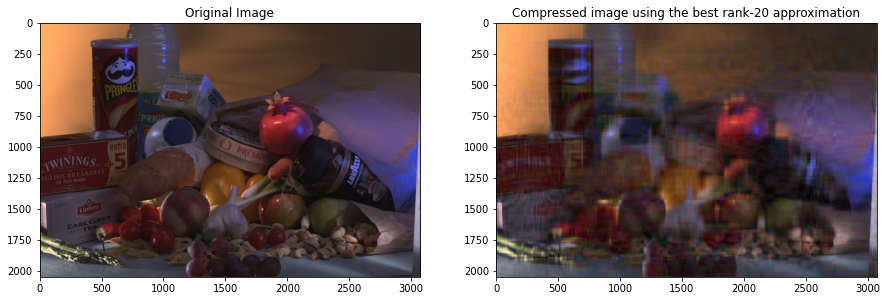
\includegraphics[width=\linewidth]{comparsion.png}
  \caption{Original and compressed images using DCT}
  \label{fig:com_dct}
\end{figure}

And then the same for each line. As a result the restored image is achieved. In Figure \ref{fig:com_dct} a reconstructed image with $z$ parameter set to $5000$, the initial size of image is $150,994,944$ bytes, of compressed image is $120,024$. So compression rate is $\sim 0.08\%$.
Below there is a complete description of the compression and decompression process, as well as calculating the compression rate using pseudocode.

\begin{algorithm}[H]
\caption{Image compression and decompressing process using DCT}\label{alg:svd}
\begin{algorithmic}

\State image \gets np.array(Image.open('hdr.ppm'))$

\State image \gets image / 255$

\State row, col \gets image.shape$

\State originalBytes \gets image.nbytes$

\State cosBackup \gets array([])$

    \For{$i \gets 0$ to $3$} 
         \State Nx, Ny \gets image.shape$
         
         \For{$line \gets 0$ to $range(Nx)$} 
         
             \State N \gets len(image[line])$
             
             \If{$len(cosBackup)$ is not N}
                \State $ret \gets zeros((N, N))$
                    \For{$n \gets 0$ to $range(len(ret))$} 
                        \For{$k \gets 0$ to $range(len(ret[n]))$} 
                           \State ret[k, n] \gets cos(((pi * k) * (2 * n + 1)) / (2 * N))$
                        \EndFor   
                    \EndFor   
                   \State cosBackup \gets ret$
             \EndIf      
             \State image \gets cosBackup.dot(image)$
             
             \State image[0] \gets image [0] * sqrt(1 / 2)$
             
             \State image[line] \gets image  * sqrt(2 / N)$
        \EndFor
        
        
        
         \For{$column \gets 0$ to $range(Ny)$} 
             \State N \gets len(image[:, column])$
             
             \If{$len(cosBackup)$ is not N}
                \State $ret \gets zeros((N, N))$
                    \For{$n \gets 0$ to $range(len(ret))$} 
                        \For{$k \gets 0$ to $range(len(ret[n]))$} 
                           \State ret[k, n] \gets cos(((pi * k) * (2 * n + 1)) / (2 * N))$
                        \EndFor   
                    \EndFor
                   \State cosBackup \gets ret$
             \EndIf
             \State image \gets cosBackup.dot(image[:, column])$
             
             \State image[0] \gets image[0] * sqrt(1 / 2)$
             
             \State image[:, column] \gets image * sqrt(2 / N)$
        \EndFor
        
    \EndFor
\algstore{bkbreak}
\end{algorithmic}
\end{algorithm}    
 
\begin{algorithm}[H]
\caption{Part 2}
\begin{algorithmic}[1]

\State imgNew \gets np.zeros(img.shape)$

\State k \gets 200$

\For{$i \gets 0$ to $range(k * 3$} 
    \State index \gets img.argmax()$
    
    \State imgNew[index] \gets img[index]$ 
    
    \State img[index] \gets 0$  
\EndFor


\State compressedDstImageBytes \gets imgNew.nbytes$   

\For{$i \gets 0$ to $range(3)$} 
    \State Nx, Ny \gets imgNew.shape$
        \For{$column \gets 0$ to $range(Ny)$} 
                \State N \gets len(imgNew[:, column])$
                \If{len(cosBackup)} is not N}
                     \State ret \gets zeros((N, N))$
                     \For{$n \gets 0$ to $range(len(ret))$} 
                        \For{$k \gets 0$ to $range(len(ret[n]))$} 
                               \State ret[k, n] \gets cos(((pi * k) * (2 * n + 1)) / (2 * N))$
                        \EndFor
                     \EndFor
                     \State cosBackup \gets ret$
                     \State imgNew[0] \gets imgNew[0] * sqrt(1 / 2)$
                     \State imgNew \gets imgNew * sqrt(2 / N)$
                     \State imgNew \gets cosBackup.T.dot(imgNew)$
                \EndIf
            \For{$line \gets 0$ to $range(Nx)$} 
                \State N \gets len(imgNew[line])$
                \If{len(cosBackup) is not N}
                    \State ret \gets zeros((N, N))$
                    \For{$n \gets 0$ to $range(len(ret))$} 
                        \For{$k \gets 0$ to $range(len(ret[n]))$} 
                           \State ret[k, n] \gets cos(((pi * k) * (2 * n + 1)) / (2 * N))$
                        \EndFor
                    \EndFor
                \EndIf
                \State cosBackup \gets ret$
                \State imgNew[0] \gets imgNew[0] * sqrt(1 / 2)$
                \State imgNew \gets imgNew * sqrt(2 / N)$
                \State imgNew[line] \gets cosBackup.T.dot(imgNew)$
            \EndFor
        \EndFor
\EndFor

    
\end{algorithmic}
\end{algorithm}

\begin{algorithm}[H]
\caption{Part 3}
\begin{algorithmic}[1]

\For{i \gets 0$ to $imgNew:$} 
    \If{imgNew[i] < 0}
        \State imgNew[i] \gets 0$
    \EndIf
    \If{imgNew[i] > 255}
        \State imgNew[i] \gets 255$
    \EndIf
\EndFor

\State decompressedImage \gets imgNew$

 \For{$i \gets 0$ to $decompressedImage$} 
    \If{decompressedImage[i] $>$ 1}
        \State decompressedImage \gets 1$
    \EndIf
    \If{decompressedImage[i] $<$ 0}
        \State decompressedImage \gets 0$
    \EndIf
\EndFor

\end{algorithmic}
\end{algorithm}

\section{Measurement Results}

\subsection{Compression Rate}

Compression rate is calculated as division of original image size to compressed image size, there is an examples of compression rate in SVD that depends on parameter $k$ on different images. The fact, that $5\%$ compression rate gives quite good picture is clearly visible.

\begin{figure}[H]
  \centering
  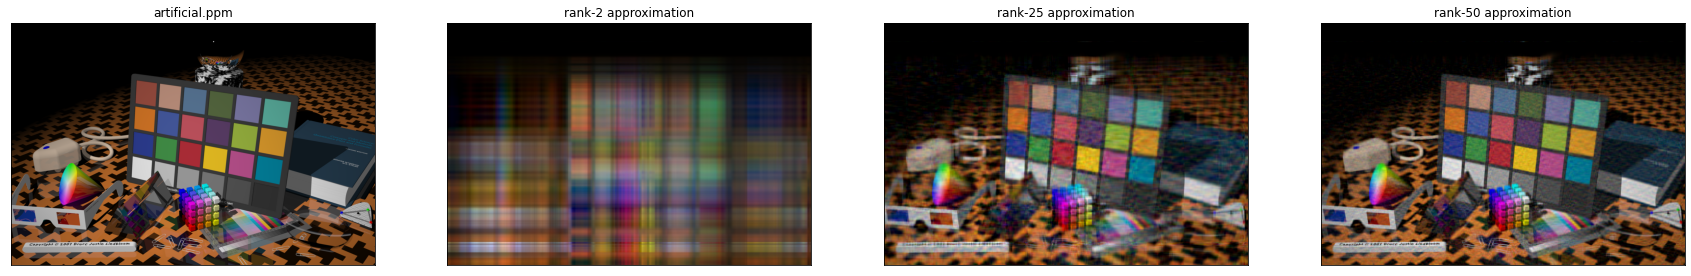
\includegraphics[width=\linewidth]{artificial_ex.png}
  \caption{Compression rate is $0.16\%$, $2.03\%$, $4.06\%$}
  \label{fig:exmp_1}
\end{figure}

\begin{figure}[H]
  \centering
  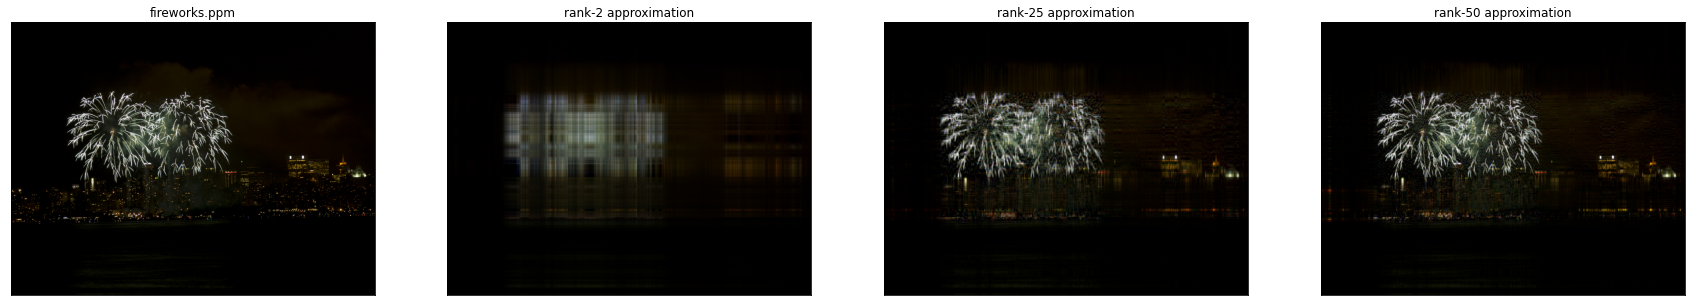
\includegraphics[width=\linewidth]{fireworks_ex.png}
  \caption{Compression rate is $0.14\%$, $1.86\%$, $3.72\%$}
  \label{fig:exmp_3}
\end{figure}

\begin{figure}[H]
  \centering
  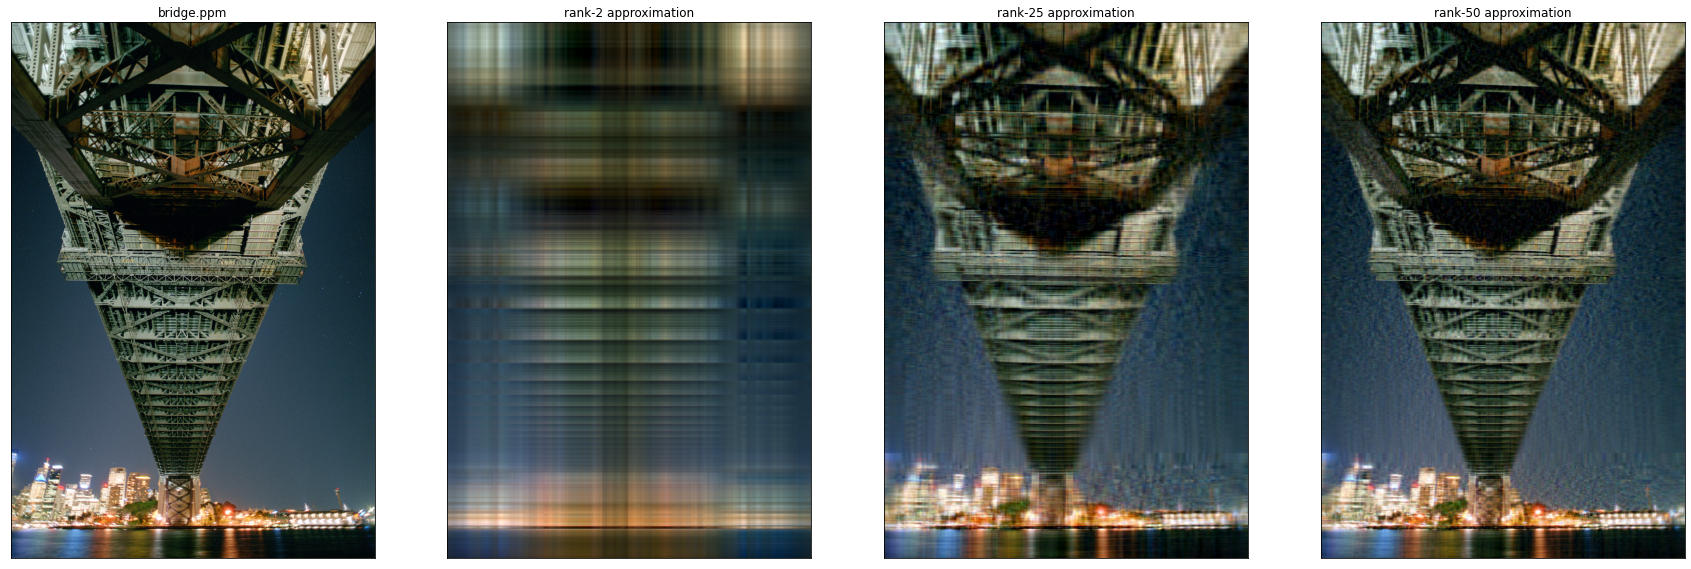
\includegraphics[width=\linewidth]{bridge_ex.png}
  \caption{Compression rate is $0.12\%$, $1.52\%$, $3.05\%$}
  \label{fig:exmp_2}
\end{figure}

\begin{figure}[H]
  \centering
  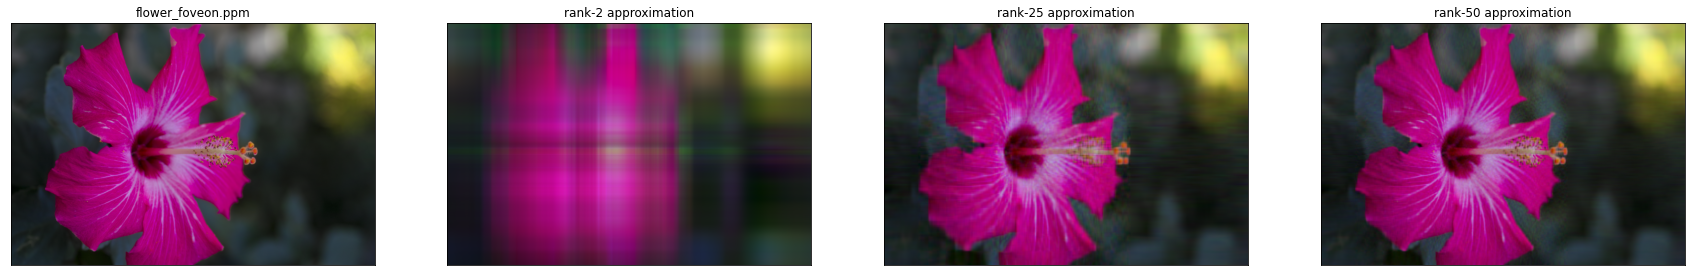
\includegraphics[width=\linewidth]{flower_foveon_ex.png}
  \caption{Compression rate is $0.22\%$, $2.75\%$, $5.51\%$}
  \label{fig:exmp_4}
\end{figure}

\begin{figure}[H]
  \centering
  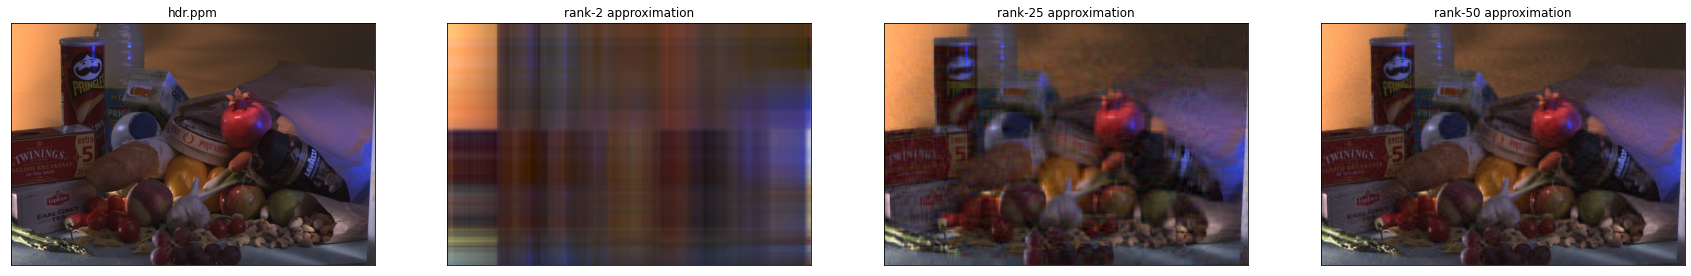
\includegraphics[width=\linewidth]{hdr.png}
  \caption{Compression rate is $0.16\%$, $2.03\%$, $4.06\%$}
  \label{fig:exmp_5}
\end{figure}

\begin{figure}[H]
  \centering
  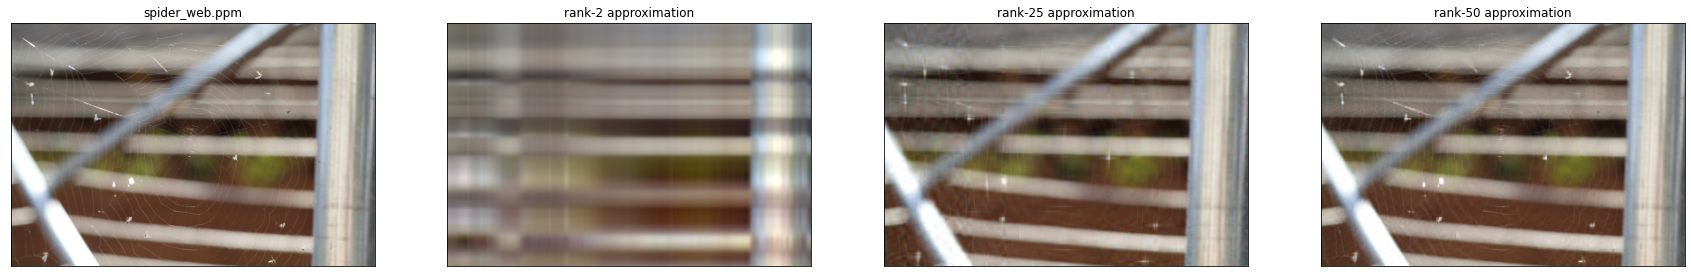
\includegraphics[width=\linewidth]{spider_web.png}
  \caption{Compression rate is $0.11\%$, $1.46\%$, $2.93\%$}
  \label{fig:exmp_6}
\end{figure}

\begin{figure}[H]
  \centering
  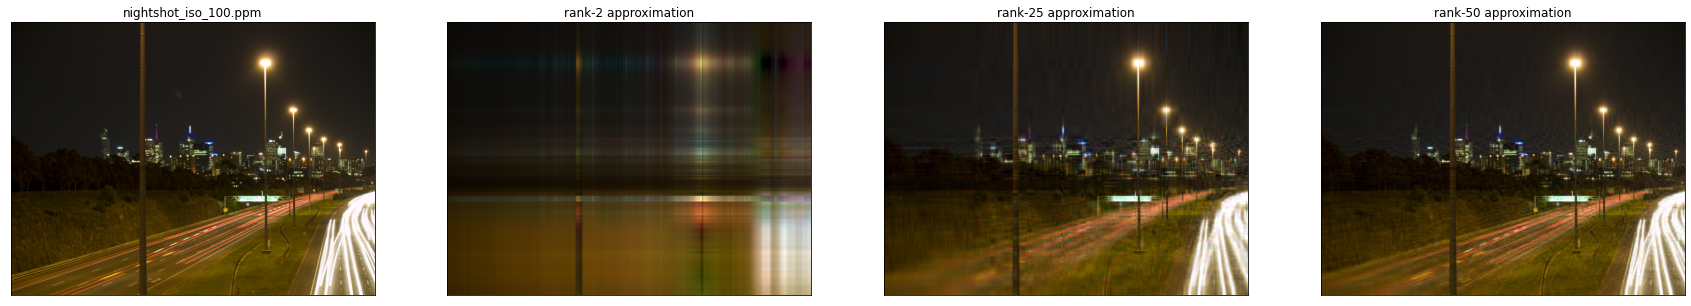
\includegraphics[width=\linewidth]{night_shot_iso_100_ex.png}
  \caption{Compression rate is $0.14\%$, $1.8\%$, $3.72\%$}
  \label{fig:exmp_7}
\end{figure}

\begin{figure}[H]
  \centering
  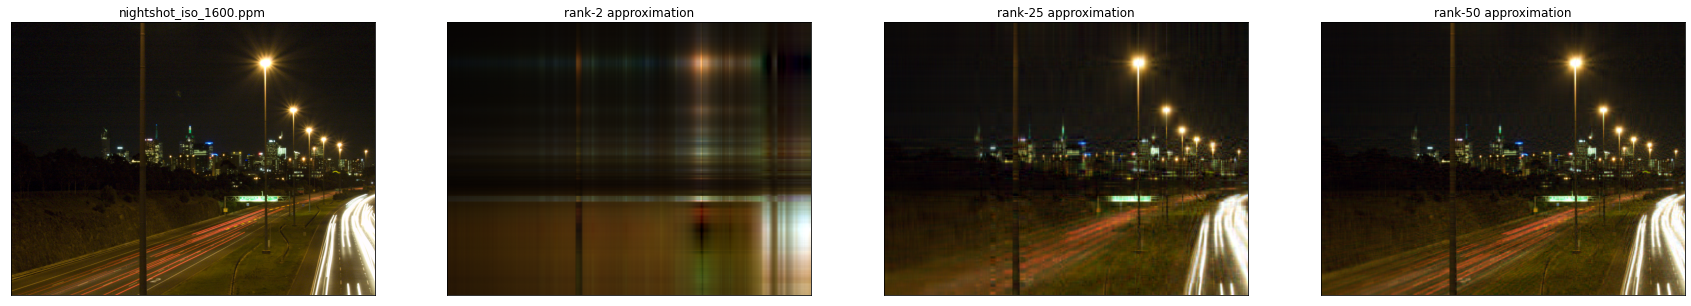
\includegraphics[width=\linewidth]{nightshot_iso_1600.png}
  \caption{Compression rate is $0.14\%$, $1.8\%$, $3.72\%$}
  \label{fig:exmp_8}
\end{figure}

Compressing by DST is demonstrating super promising results, image without visible differences from original is achieved with $0.292\%$ compression rate. 

\begin{figure}[H]
  \centering
  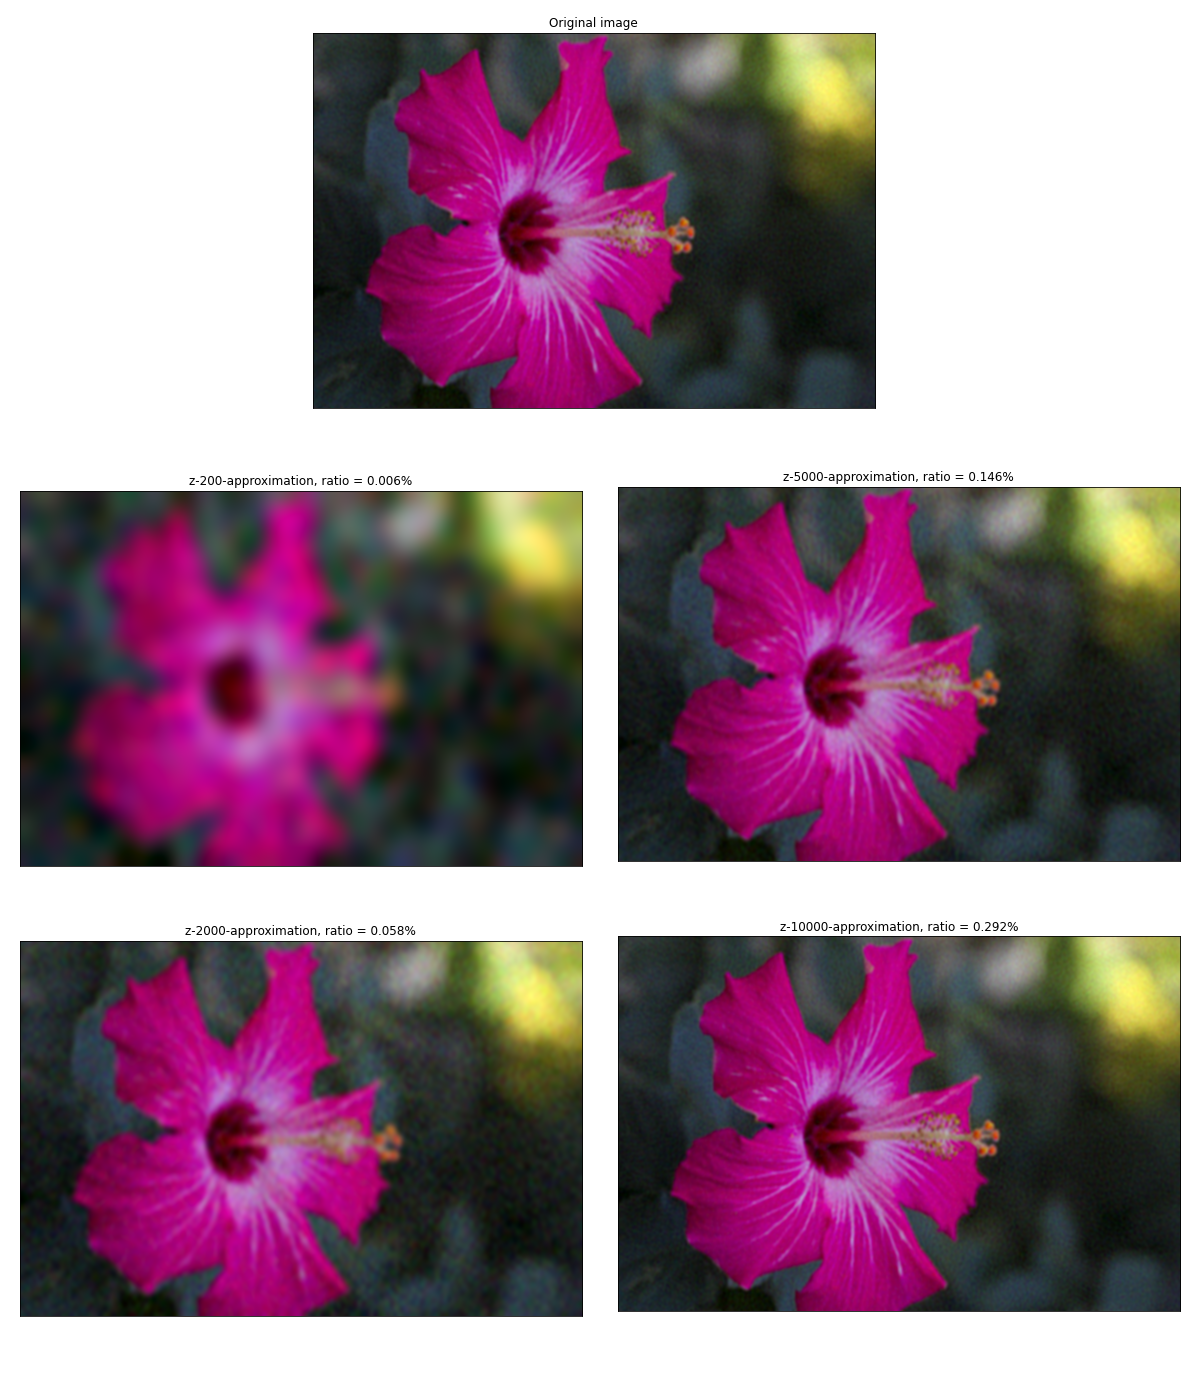
\includegraphics[width=0.9\linewidth]{dst_benchmark_1.png}
  \caption{Compression rate is $0.005\%$, $0.058\%$, $0.14\%$ and $0.29\%$}
  \label{fig:exmp_9}
\end{figure}

\subsection{Quality}

Below are the results of measurements in the pictures using SVD. It can be seen that the SIM metric works better, because we know that acceptable picture quality is achieved at a compression rate of 3-4 percent, and for this SSIM rate, the result shows better results. You can also notice how the graph changes if you pay attention to 2 pictures with different ISO, you can see that compression works better on a photo with a low ISO.

\begin{figure}[H]
  \centering
  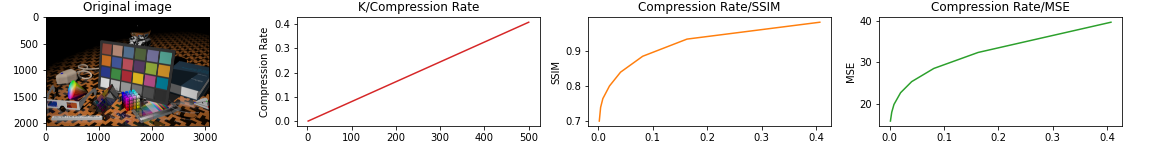
\includegraphics[width=\linewidth]{articial.png}
  \label{fig:exmp_10}
\end{figure}

\begin{figure}[H]
  \centering
  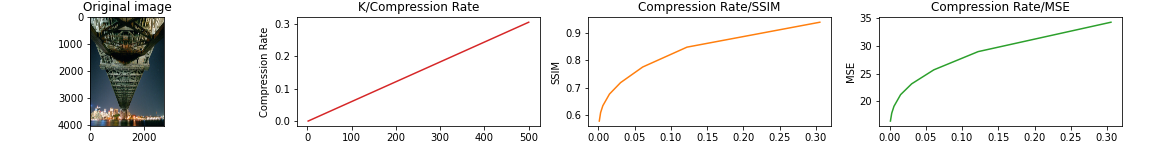
\includegraphics[width=\linewidth]{Bridge.png}
  \label{fig:exmp_11}
\end{figure}

\begin{figure}[H]
  \centering
  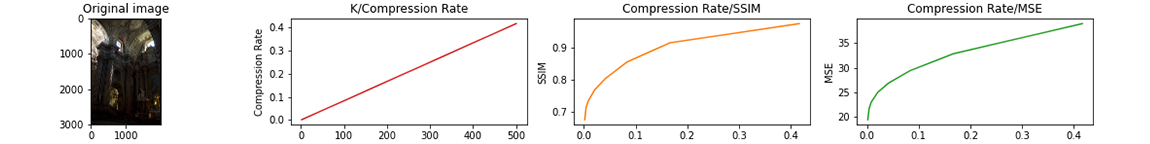
\includegraphics[width=\linewidth]{Cathedral.png}
  \label{fig:exmp_12}
\end{figure}

\begin{figure}[H]
  \centering
  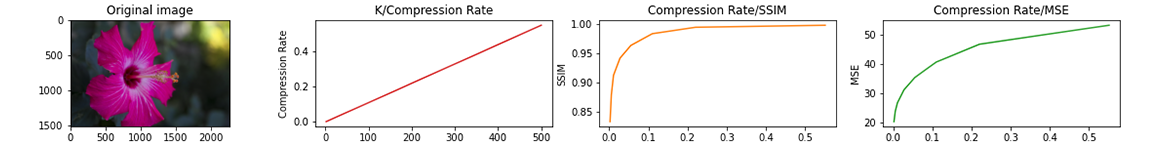
\includegraphics[width=\linewidth]{Flower Foveon.png}
  \label{fig:exmp_13}
\end{figure}

\begin{figure}[H]
  \centering
  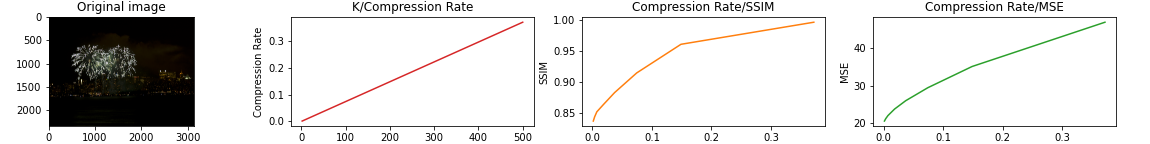
\includegraphics[width=\linewidth]{Fireworks.png}
  \label{fig:exmp_14}
\end{figure}

\begin{figure}[H]
  \centering
  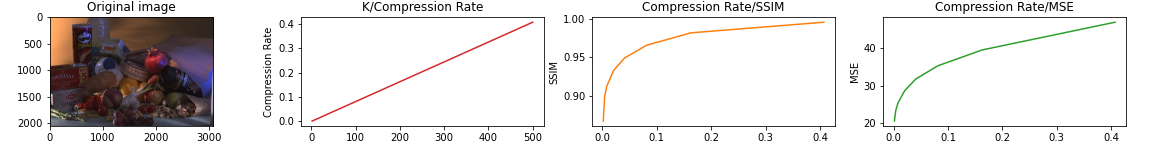
\includegraphics[width=\linewidth]{HDR (1).png}
  \label{fig:exmp_15}
\end{figure}

\begin{figure}[H]
  \centering
  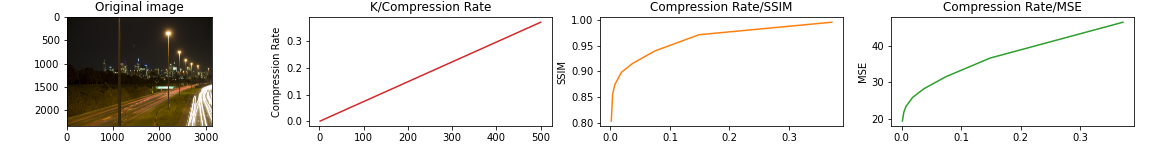
\includegraphics[width=\linewidth]{Nightshot ISO 100.png}
  \label{fig:exmp_16}
\end{figure}

\begin{figure}[H]
  \centering
  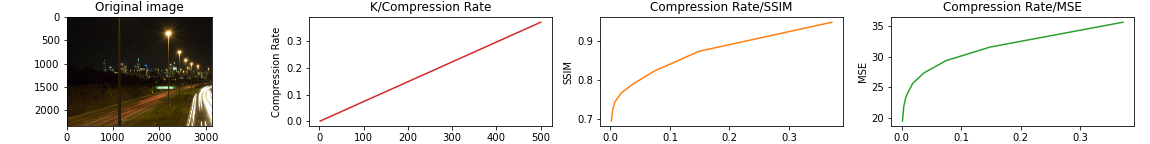
\includegraphics[width=\linewidth]{Nightshot ISO 1600.png}
  \label{fig:exmp_17}
\end{figure}

\begin{figure}[H]
  \centering
  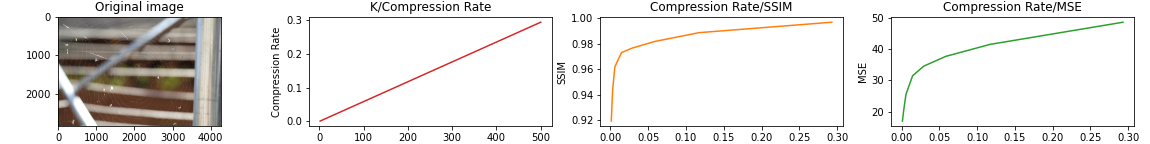
\includegraphics[width=\linewidth]{Spider-web.png}
  \label{fig:exmp_18}
\end{figure}

There is also a comparison of the compression quality of SVD  and DST (DCT is first picture, SVD is second one), which shows that the same quality is achieved with a compression rate of $0.25\%$ and $0.0015\%$ for the corresponding algorithms, that is, DCT compresses $150$ times better with the same quality of a compressed image.

\begin{figure}[H]
  \centering
  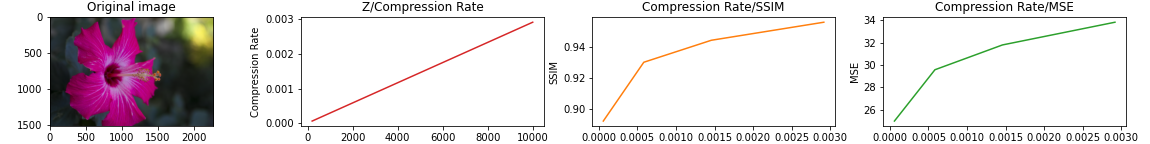
\includegraphics[width=\linewidth]{flower-dct.png}
  \label{fig:exmp_19}
\end{figure}

\begin{figure}[H]
  \centering
  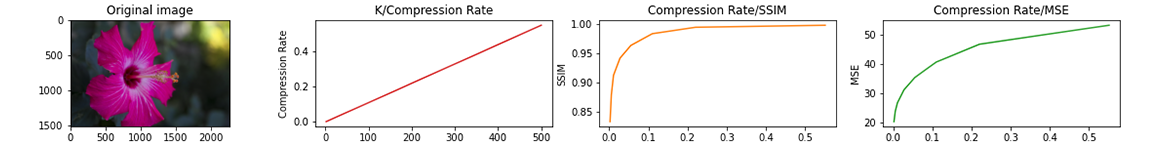
\includegraphics[width=\linewidth]{Flower Foveon.png}
  \caption{Comparing between DCT and SVD}
  \label{fig:exmp_13}
\end{figure}

\subsection{Time Complexity}

DCT showed better quality than SVD, but also took a lot longer to compress. On average, SVD took $3$ minutes, of which $90\%$ of the time is taken up by the compression process due to the SVD part. And the DCT took an average of $13$ minutes - $65\%$ for the compression process and $35\%$ for the decompression. Below are suggestions why DCT runs much longer than SVD: SVD was used as a built-in library solution, and DCT was written from scratch, time degradation occurred due to insufficient optimization. A Fourier Transform was also used, which has $O(N^2)$ complexity, but real compression algorithms use an accelerated version - Fast Fourier Transform (FFT), which has $O(N log N)$ complexity, which is a significant speedup. It also makes sense to hypothesize that with all these optimizations, the DCT will still not reach the performance of SVD due to the presence of a high quality trade off, but also requires additional verification.

\section{Conclusion}
One of the more interesting parts of this was comparing how the decrease in
image quality manifested itself between the two image compression techniques.
There is a clear difference in how the low quality SVD compressed images are
distorted versus how the low quality DCT compressed images were distorted.
Another interesting difference was how DCT had a much higher compression
ratio than the SVD compression, with the result images having similar image
quality. The final compression ratio for DCT was about 30 times higher. The
graph below shows a comparison between SVD and DCT for the various k values
tested. While the techniques for this project were explored using a grayscale image,
all of the above could easily be applied to a RGB or RGBA image to further
explore the topic. It would be interesting to see how the additional dimension
of color affects the compression algorithms and compression ratios.

\end{document}